\subsection{Diagrammi di sequenza}
\begin{figure}[hb]
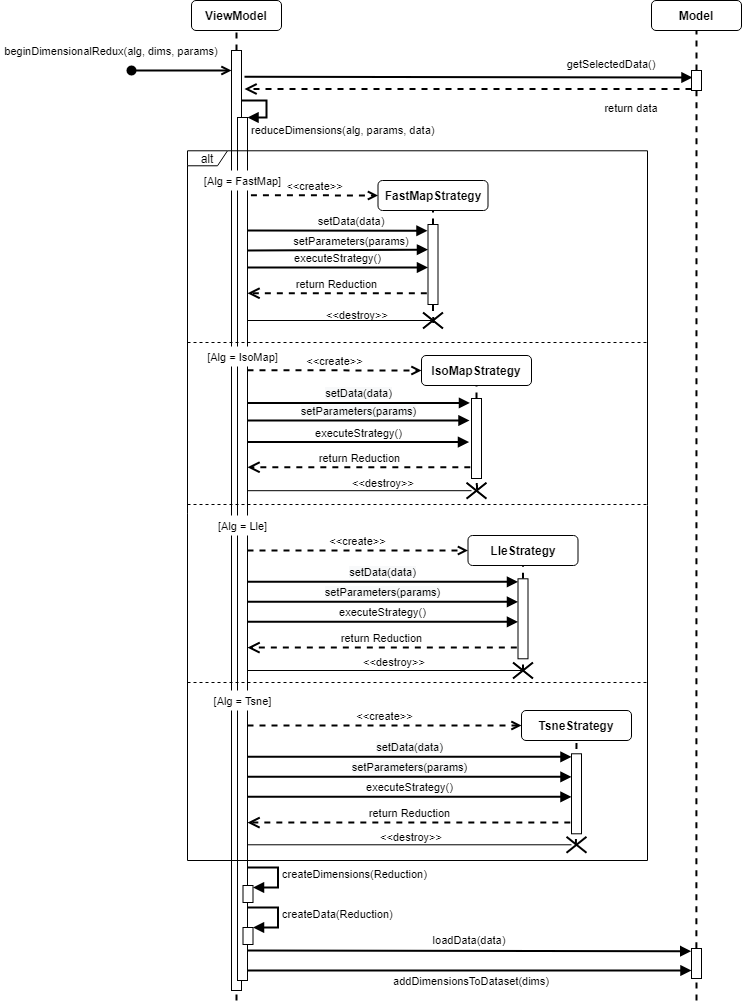
\includegraphics[width=12cm]{Images/Allegato Tecnico-Sequenza-DR}
\centering
\caption{Diagramma di sequenza che modella il processo di riduzione dimensionale}
\end{figure}
La funzione \texttt{beginDimensionalRedux()} è la funzione chiave per la riduzione dimensionale dei dati. Essa viene chiamata nel \textit{ViewModel} mentre l'utente interagisce con l'UI. Da qui il \textit{ViewModel} ottiene i dati dal \textit{Model} memorizzandoli nell'oggetto "data" per poi utilizzarli nella relativa \glo{Strategy} (a seconda dell'algoritmo di riduzione scelto), alla quale vengono passati, oltre ai dati, i paramatri relativi all'algoritmo settati dall'utente.
Vengono quindi ritornati i dati ridotti e inseriti in array tramite i metodi \texttt{createDimensions()} e \texttt{createData()}, che verranno successivamente aggiunti al dataset iniziale.
\newpage
\begin{figure}[hb]
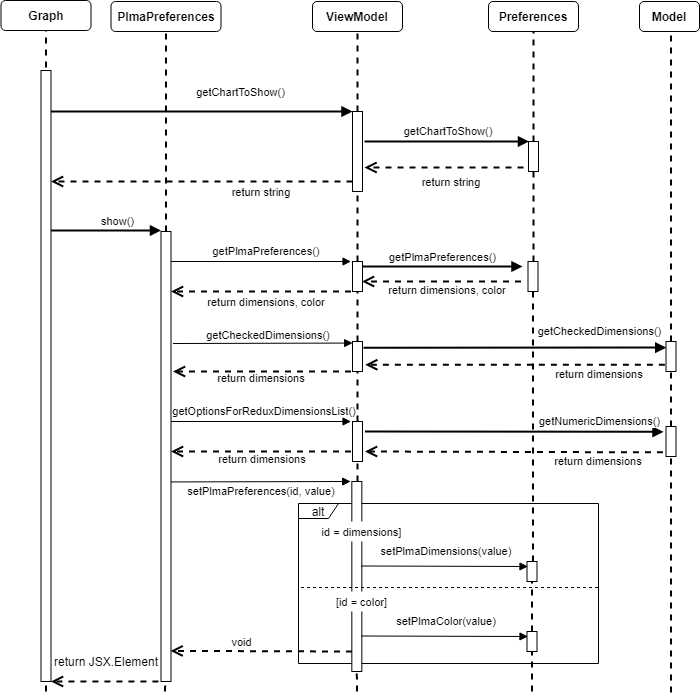
\includegraphics[width=14cm]{Images/Allegato Tecnico-Sequenza-PLMApref}
\centering
\caption{Diagramma di sequenza che modella il processo di visualizzazione del box di preferenze per il grafico PLMA}
\end{figure}
Per semplicità è stato preso come esempio un singolo tipo di grafico. Per la visualizzazione dei box di \glo{preferenze} per gli altri grafici vale lo stesso schema di funzionamento.
La funzione \texttt{getChartToShow()} viene chiamata ogni volta che nel modello avvengono delle modifiche. Questa funzione ritorna una stringa con il nome del tipo di grafico da visualizzare, in questo caso conterrà "PLMA".
Successivamente viene chiamata la funzione \texttt{show()} per mostrare a video un box con le preferenze scelte. Quest'ultimo chiama varie funzioni del \textit{ViewModel}:
\begin{itemize}
\item \texttt{getPlmaPreferences()}, la quale ritorna le preferenze salvate nella classe Preferences;
\item \texttt{getCheckedDimensions()}, la quale ritorna le dimensioni scelte, salvate nel \textit{Model};
\item \texttt{getOptionForReduxDimensionsList()}, la quale ritorna le dimensioni scelte e non categoriche (necessarie per il \glo{PCA}), salvate nel \textit{Model};
\item \texttt{setPlmaPreferences()}, la quale salva le preferenze settate dall'utente nella classe Preferences.
\end{itemize}
\newpage
\begin{figure}[hb]
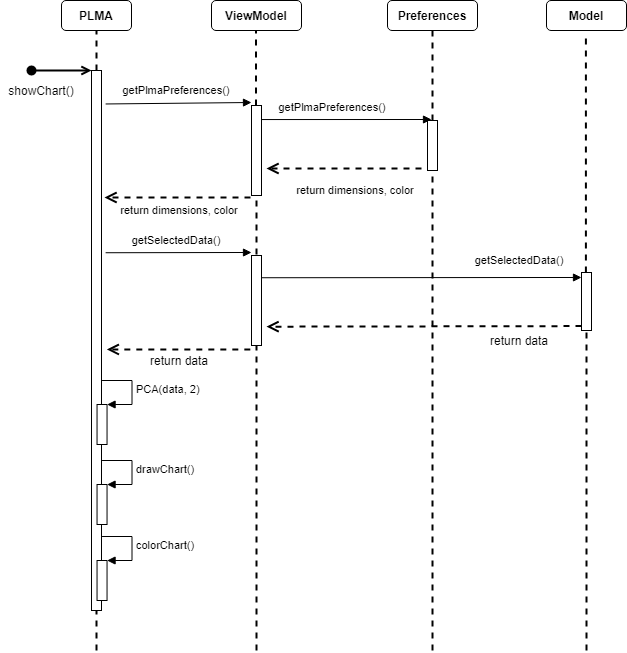
\includegraphics[width=15cm]{Images/Allegato Tecnico-Sequenza-PLMA}
\centering
\caption{Diagramma di sequenza che modella il processo per la visualizzazione del grafico PLMA}
\end{figure}
Anche in questo per semplicità è stato preso come esempio un singolo tipo di grafico. Per la visualizzazione degli altri grafici vale lo stesso schema di funzionamento.
\texttt{showChart()} è la funzione principale per richiamare la costruzione di un grafico, inizialmente vengono lette le preferenze settate dall'utente grazie al metodo \texttt{getPlmaPreferences()}, e vengono letti i dati da visualizzare grazie al metodo \texttt{getSelectedData()}. Successivamente viene invocato il \glo{PCA} per avere le coordinate di partenza dei punti nel grafico (necessario per la visualizzazione del grafico PLMA). Infine il grafico viene disegnato tramite il metodo \texttt{drawChart()} e i punti vengono colorati tramite il metodo \texttt{colorChart()}.

\newpage